\chapter{Theoretical Background}\label{ch:theory}

This chapter introduces concepts and terms used throughout the work. It starts with a general discussion of \gls{ai} and common terms used in this field. Second part discusses \glspl{nn} as its the main \gls{ml} model used in this theses. The next section describes \gls{cnn}, a special type of \gls{nn} widely used in image processing. The last part introduces the Kalman filter.

\section{Artificial Intelligence}

There are many definitions of \gls{ai}. \cite{modernApproach} define \gls{ai} as the study of agents that receive percepts from the environment and perform actions. Each such agent implements a function that maps percept sequences to actions. Other possibilities are to define \gls{ai} as the study of either intelligent or human-like systems.

Another term associated with \gls{ai} is \gls{ml}, an area of \gls{ai} that focuses on automatic learning of correct actions based on data.  Another way to look at this is that the system autonomously gains knowledge from training data. There are two main approaches in \gls{ml} - \textit{supervised learning} and \textit{unsupervised learning}. 

In unsupervised learning, the model is trying to gain information from the dataset without explicit correct answers. The absence of correct answers leads to difficulties when evaluating the results but further reduces the need for human input. Typical tasks in unsupervised learning are based on clustering.

Supervised learning uses datasets with correctly labeled data. The availability of labels leads to a straightforward approach where the model can optimize some function related to how much its output matches the labels. The optimized function is often called \textit{loss function}, \textit{objective function} or \textit{cost functions}.

\subsection{Supervised Learning}

This part introduces common concepts and approaches in supervised learning.

Main tasks of supervised learning are \textit{classification} and \textit{regression}. Both deal with assigning a value to some input vector. In classification, the task is to assign a label from a finite and typically small number of choices called classes. In regression, the number of possible answers is infinite, or it is practical to state the problem as if there was.

The typical supervised learning process splits the dataset into three parts. The first part is called \textit{training} data and is used to train the model. Second part is \textit{evaluation} data. The evaluation data is used to evaluate the performance of a trained model. The main goal of this evaluation is to find \textit{hyperparameters}. Hyperparameters are parameters that the model does not learn on its own during training. The last part of the dataset is called \textit{testing} data. It is used in the final stage to evaluate the model on data it has not seen yet. This evaluation enables reasonably predicting the model's performance on future data, assuming that the testing dataset is representative.

Alternative method for finding hyperparameters is \textit{cross-validation}. Instead of splitting the dataset into fixed training, evaluation, and testing parts, the data is split only into training and testing data. Training data is then split into $n$ parts. In each training step, we train the model $n$ times on the training data without one part (in a way to leave out each part once). This approach can lead to more robust models and is especially useful when the dataset is relatively small. On the other hand, this increases the computing time significantly.

%% Technically subcategory of AI but I feel like shallow structures are better - is it ok like this?
\section{Neural Networks}
Artificial Neural Network is a model that is used throughout this work. \Glspl{nn} have proved to be very useful, especially in the area of image processing. There are many types of \glspl{nn}, and their use is very versatile. This section provides a basic introduction to \glspl{nn}. 

A basic part of \gls{nn} is a neuron. An artificial neuron is a model that is inspired by a biological neuron. However, while the workings of a biological neuron are complicated, the artificial neuron is very simple. The main idea is that many simple units linked together can add up to an intelligent whole. 

\subsection{Artificial Neuron}

Output of a single neuron is calculated as some function, called \textit{activation function} applied to a weighted sum of inputs as shown in \autoref{e:neuron}, where $x_i$ is the $i$-th input, $w_i$ its weight, $b$ is the bias, $\sigma$ is the activation function and $n$ is the number of inputs.

\begin{equation}
    \label{e:neuron}
    y = \sigma\left(\sum_{i=1}^n (w_ix_i) + b\right)
\end{equation}

\subsection{Activation Functions}
The activation function should be nonlinear. Linear functions are not useful here because the composition of linear functions is a linear function, so we could easily replace multiple neurons with one neuron with different weights. Non-linearity is also needed to fit nonlinear data. 

Activation functions are usually required to be differentiable. The differentiability is needed for \textit{backpropagation} algorithm, which is an algorithm for efficient training of \glspl{nn} that will be introduced later.

Common activation functions are:
\begin{itemize}
    \item sigmoid: $\sigma(x) = \frac{1}{1+e^{-x}}$,
    \item hyperbolic tangent: $\tanh(x) = \frac{e^{2x}-1}{e^{2x}+1}$,
    \item ReLU: $\text{ReLU}(x)=\max(0, x)$.
\end{itemize}



The last layer typically uses different activation functions based on the target task. For binary classification the typical function is \textit{logistic sigmoid}
$$f(\xi) = \frac{1}{1 + e^{-\xi}} = \frac{e^\xi}{1 + e^\xi}$$
and the resulting value is interpreted as the probability that the given input is from class 1. This can be written as $\hat{\pst}(Y=1|X=x).$

For classification into $c$ classes a \textit{softmax} function is used with $c$ output neurons. Output for $i$-th neuron is
$$
f_i(\xi) = \frac{e^{\xi_i}}{e^{\xi_1} + \hdots + e^{\xi_c}},
$$
where $\xi = (\xi_1, \hdots, \xi_c)^T$ and $\xi_i$ is the input for $i$-th output neuron. The interpretation is similar as for the binary case, formally $f_i(\xi) = \hat{\pst}(Y=i|X=x)$. Final prediction is then the class with maximum probability assigned
$$
\hat{Y} = \argmax_{i \in 1,\dots{},c} f_i(\xi).
$$

\subsection{Feed Forward Neural Network}\label{s:feed-forward}

A feedforward neural network is a basic type of \gls{nn} with neurons organized into layers. The first layer is called \textit{input layer} and represents input variables. Last layer is called \textit{output layer}. The remaining layers are called \textit{hidden layers}. 

\glspl{nn} with large number of hidden layers are sometimes called \textit{deep neural networks}. Usage and study of such \glspl{nn} is sometimes called deep learning. There is however no consensus on the precise meaning of the term. In practice, the term deep learning is often synonymous with learning of \glspl{nn}.

Every neuron in each layer is connected to neurons in the following layers creating a directed acyclic graph. 

\begin{figure}[ht]
\centering
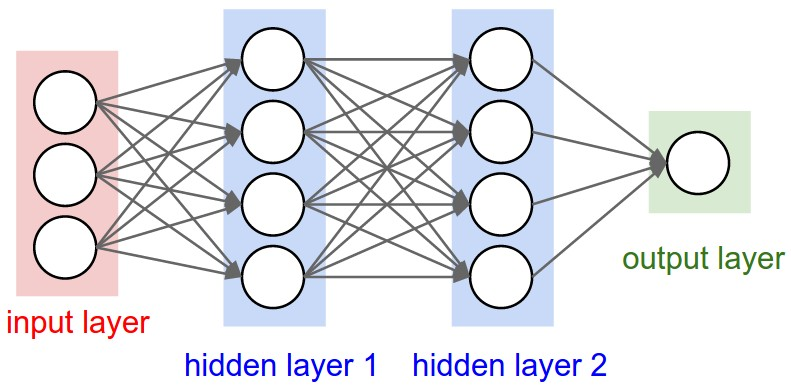
\includegraphics[width=0.5\textwidth]{neural_net}
\caption[Structure of a simple neural network.]{Structure of a simple neural network.\cite{cs231n}}
\label{fig:nn1}
\end{figure}

Let $w^l_{i,j}$ be the weight of connection from $i$-th neuron in $(l - 1)$-th layer to $j$-th neuron in $l$-th layer. Let $b_j^l$ be the bias of $j$-th neuron in $l$-th layer, $\sigma$ some activation function and $N^{(l)}$ number of neurons in layer $l$. Then the activation (output) $a_j^l$ for the $j$-th neuron in $l$-th layer is
\begin{equation}
    \label{e:activation}
    a^l_j = \sigma \left( \sum_{i=1}^{N^{(l-1)}} (w_{i,j}^l a^{l-1}_i) + b_j^l \right).
\end{equation}

We can write this more succinctly with the usage of matrices and vectors. Let $W^l$ be a weight matrix for layer $l$ which has $w^l_{i,j}$ from \autoref{e:activation} in $j$-th row and $i$-th column. Similarly let $b^l = (b_1^l, \dots{}, b_{N^{(l)}}^l)$ be a bias vector. Then we can compute an activation vector $a^l$ whose components are activations $a_j^l$ with
\begin{equation}
    \label{e:layerActivation}
    a^l = \sigma\left( W^la^{l-1} + b^l \right)
\end{equation}

Each layer produces a nonlinear transformation of outputs from previous layers. \cite{hornik} proved that standard multilayer feedforward networks with as few as one hidden layer are capable of approximating any Borel measurable function from one finite-dimensional space to another to any desired degree of accuracy. In this sense, multilayer feedforward networks are universal approximators. However, finding parameters for such networks is rather difficult.

\cite{bengio2007scaling} argues that shallow architectures can be very inefficient in terms of the required number of computational elements and examples. Furthermore, they argue that deep architectures have the potential to generalize in a way that is crucial to make progress on the kind of complex tasks required for artificial intelligence. This corresponds well with empiric observations. Commonly used \glspl{nn} have tens of layers and millions of parameters \cite{mobilenets, osnet, yolo}.

\subsection{Learning}

The goal of learning is to find the parameters $\theta = (W,b)$ (from \autoref{e:layerActivation}) that minimize the selected loss function $L(\theta)$.  Common loss functions are categorical cross-entropy for multi-class classification and \gls{mse} for regression.

Let $\theta$ be learned parameters, $Y$ the vector of target labels, also called \textit{ground truth}, and $\hat{Y}$ vector of predicted values from \gls{nn} based on $\theta$ and $N$ input vectors. Let $||.||$ be L2 norm. Then \gls{mse} is defined as:

\begin{equation}
    \label{e:mse}
    L(\theta) = \frac{1}{N} \left|\left|Y - \hat{Y}\right|\right|.
\end{equation}

With the use of a suitable cost function such as \gls{mse} and differentiable activation functions the whole \gls{nn} is differentiable and can be trained using \textit{backpropagation}. 

Backpropagation is an iterative algorithm, where we compute the gradient of the cost function with respect to the weight and then update the weights with a step proportional to the negative of the gradient. The algorithm is explained in more detail, for example in \cite{werbos1990backpropagation}.


\section{Convolutional Neural Networks}\label{s:cnns}

This section introduces \glspl{cnn}, which are a specialized kind of \gls{nn} for processing data with a known grid-like structure, for example, time-series data or images. Convolutional networks have been very successful in practical applications. The information in this section is mainly based on \cite{Goodfellow-et-al-2016} and \cite{cs231n}.

\Gls{cnn} is a \gls{nn} that uses \textit{convolution} instead of general matrix multiplication in at least one of its layers.  Convolution is a mathematical operation defined for functions $f$ and $g$ as
$$
(f * g)(t) = \int_{-\infty}^\infty f(x)\, g(t - x)\, dx
$$
in continuous and
$$
(f * g)(t) = \sum_{a=-\infty}^\infty f(a)\, g(t - a)
$$
in the discrete case. The first argument $f$ is called \textit{input} and the second argument $g$ is called \textit{kernel} of the convolution. The output is sometimes referred to as the \textit{feature map}. Convolution can be generalized to multiple dimensions.

In machine learning applications, the input is usually a \textit{tensor} (multidimensional array) of data, and the kernel is usually a tensor of learned parameters. In practice, both input and kernel are considered zero everywhere but in the finite set of points where we store their values. This allows the implementation of the infinite summation as a summation over a finite number of elements.

In traditional neural networks, the neurons in each layer are connected to all neurons from the previous layer. This large number of connections leads to a large number of parameters that need to be learned. \Glspl{cnn} leverage the structure of input data to reduce the number of parameters. If we assume that the input consists of images, we can reasonably constrain the neural network architecture.

The layers of \glspl{cnn} are arranged in three dimensions: width, height, and depth (which refers to the third dimension of an activation volume). The input layer holds the image, so its width and height will be the dimensions of the image, and the depth would be three for color images (representing the three \gls{rgb} channels).

\begin{figure}[ht]
\centering
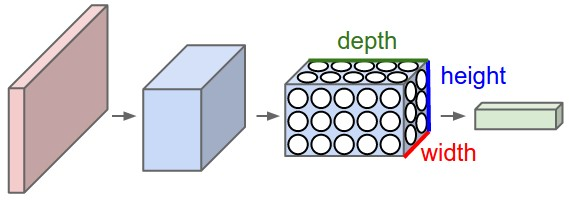
\includegraphics[width=0.5\textwidth]{cnn_3d}
\caption[\acrshort{cnn} layer transformation of 3D input volume to 3D output volume.]{\Gls{cnn} layer transformation of 3D input volume to 3D output volume.\cite{cs231n}}
\label{fig:cnn_transform}
\end{figure}

Three main types of layers are used to build \glspl{cnn}: \textit{convolutional layer}, \textit{pooling layer} and \textit{fully-connected layer}. Fully-connected layers were already introduced in section \ref{s:feed-forward}.

\subsection{Convolutional Layer}

A convolutional layer is the core building block of \gls{cnn}. Each layer consists of a set of learnable \textit{filters}. Every filter is spatially small and has the depth of the input volume. Each filter is convolved across the input volume's width and height to produce a two-dimensional activation map. Intuitively, the network will learn filters that activate when they see some feature. The idea is that early layers learn to recognize simple features like an edge, and later layers will learn to recognize more complicated patterns based on these features. The output of the whole convolutional layer is the output of each filter in given layers stacked along the depth dimension - this produces the output volume. 

Every entry in the 3D output volume can be interpreted as an output of a neuron looking at only a small region in the input and sharing parameters with all the neurons that apply the same filter. This property is called \textit{local connectivity}.

The spatial extent of this connectivity is determined by a hyperparameter called \textit{filter size}. The filter size only affects the spatial dimensions (width and height). The connectivity along the depth axis is always equal to the depth of the input volume.

Convolutional layers use a schema called \textit{parameter sharing} to reduce the number of parameters greatly. This reduction is based on the assumption that if one feature is useful to compute at some spacial position $(x,y)$, it should also be useful to compute at different positions. We can then constrain the neurons in each depth slice to use the same weights and bias. It is common to refer to this shared set of weights as a \textit{filter} (or a \textit{kernel}).

\subsection{Pooling Layer}

Pooling layers perform non-linear downsampling of the input. They do this by combining multiple values into a single value that they pass to the next layer. Most common approach is \textit{max pooling}. Max pooling takes the maximum value from its input.

It is common to periodically insert a pooling layer between convolutional layers in a \gls{cnn} architecture. The layer's function is to reduce the number of parameters, which reduces the number of computations needed and helps control overfitting.

\subsection{Transfer Learning}

\textit{Transfer learning} is a standard process, where we take a pre-trained model for a similar task and use it as initialization or a feature extractor for the target task. The use of pre-trained models dramatically reduces the computational power needed and the need for an extensive dataset.

The use of an existing \gls{cnn} as a feature extractor is simple, as only the last fully-connected layer needs to be removed or replaced.

\section{Kalman Filter}\label{s:kalman}

This section introduces \textit{Kalman filter}, which is an integral part of tracking algorithms used in this work. The information in this section is mainly based on \cite{labbe2014}.

Kalman filter is a mathematical model to gain (relatively) precise information about a system based on imprecise measurements and information about the system. Kalman filters are fairly general and have usages in estimation, data smoothing, and control applications. We will focus mainly on its usage in tracking applications.

\subsection{Introduction to g-h Filters}

Any real measurement is inaccurate. The output of any sensor does not give us perfect information about the observed system but depends on the sensor's quality. To deal with this, we can use an algorithm called \textit{g-h filter} (also called alpha-beta filter).

The first idea of the g-h filter is that the system's behavior should influence how we interpret the measurements. Imagine we are weighting a rock and getting slightly different results each time. We would probably attribute these differences to noise in the measurement. On the other hand, if we were getting changing position from a car GPS, we might conclude that the car is moving.

Assume we have some predictions for the target variable.  If we only form estimates from the measurements, then the prediction will not affect the result. If we only form estimates from the prediction, then the measurements will be ignored. This leads to the second idea that we need to take some combination of the prediction and measurement. We will call the difference between the measurement and prediction the \textit{residual}. 

In general, we cannot expect to know the rate of change of the target variable, and it also may change over time. These ideas lead to an iterative two-step process. First, we \textit{predict} the target variable and its rate of change. Next, we \textit{update} the target variable and its rate of change based on the prediction and new measurement.

This algorithm is very general. Kalman filter is then one approach on how to do these steps.

\subsection{Kalman Filter Algorithm}

Like any g-h filter, the Kalman filter makes a prediction, reads a measurement, and then forms a new estimate between the two.

The Kalman filter is using normal distributions for the representation of measurements and predictions. The normal distribution is well studied and has many interesting properties. Using normals allows us to store information about whole probability distribution as just two numbers - mean $\mu$ and variance $\sigma^2$.

Sum of two normal distributions $N(\mu_1, \sigma^2_1), N(\mu_2, \sigma^2_2)$ is a normal distribution $N(\mu_1 + \mu_2, \sigma^2_1 + \sigma^2_2)$. The product of two normal distributions is proportional to a normal distribution, meaning we can scale it to a normal distribution. These two properties mean we can sum and multiply normal distributions, and the result will still be a normal distribution (assuming we are normalizing after multiplication). 

\subsubsection*{Predict}

The general formula for the predicting the next state mean is
\begin{equation}\label{e:predict_mean}
    \overline{x} = Fx + Bu.
\end{equation}
$x$ denotes the state mean. $F$ is the \textit{state transition function}. $B$ and $u$ let us model control inputs to the system and can be removed if we do not have any control over it.

State covariance $\overline{P}$ is predicted with
\begin{equation}\label{e:predict_covar}
    \overline{P} = FPF^T + Q,
\end{equation}
where $P$ is the previosu state covariance, $F$ is the state transition function from \autoref{e:predict_mean} and $Q$ is the process covariance.

\subsubsection*{Update}

The update step consists of applying the following equations.

\begin{align}
    y &= z - H\overline{x} \\
    K &= \overline{P}H^T(H\overline{P}H^T + R)^{-1} \\
    x &= \overline{x} + Ky \\
    P &= (I - KH)\overline{P}
\end{align}

$\overline{x}, F$ and $\overline{P}, Q$ are from equations \ref{e:predict_mean} and \ref{e:predict_covar} respectively. $H$ is the measurement function. $z$ and $R$ are the measurement mean and \textit{noise covariance}. $K$ is called \textit{Kalman gain}. $I$ is the identity matrix.

Measurement noise is the variance of the sensor we are using, while process noise is the observed system variance. The measurement function maps the true state space into the observed space. 
The Kalman gain is the relative weight given to the measurements and current state estimate. With a high gain, the filter places more weight on the most recent measurements.


\subsubsection*{Summary}

\textit{Kalman filter} is a recursive algorithm that can be used to extract useful information from noisy measurements.

In the context of tracking, the Kalman filter can be used to better approximate track's bounding boxes. The Kalman state is typically some representation of a rectangle and its speed. The measurements are usually taken from a \gls{cnn}. These measurements are noisy, and the Kalman filter smooths them to provide a more accurate and stable position. Furthermore, we can also predict the track's position in the next frame, which is used to match the track to new detections. 

The filter needs correctly designed models and functions introduced in previous sections to work correctly. There is no universal approach, and the design must be based on experience, intuition, and experimentation. One possible design is described in section \ref{s:kalman_design}.
